
\fullcite{bepo10}

This is in my opinion a fantastic article. 
Physics is explained, FEM discretisation is derived, 
with benchmarks and experiments.


\fbox{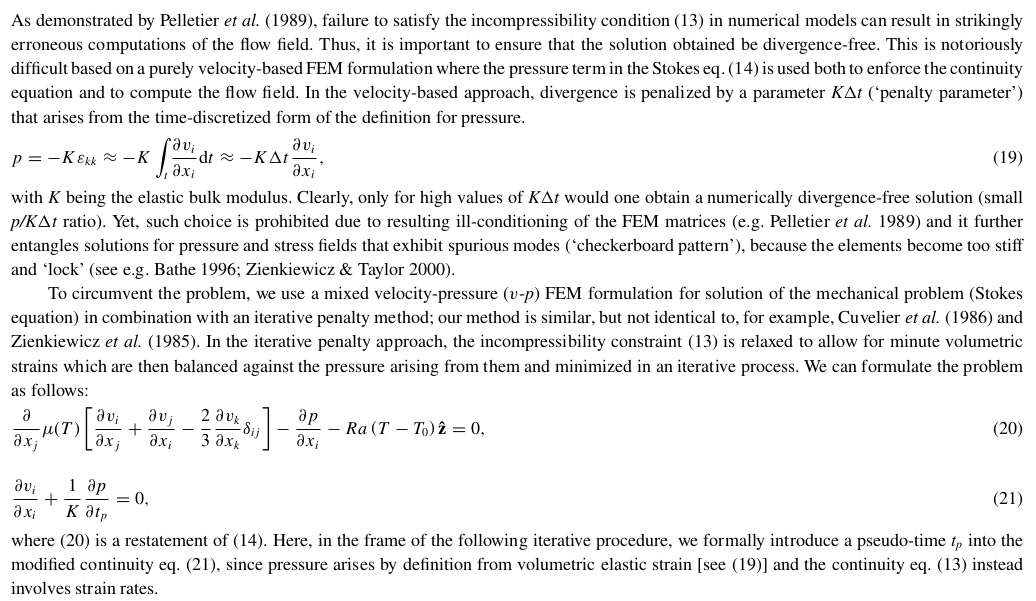
\includegraphics[width=15cm]{images/viscoelasticity/bepo10_a}}

\[
p=-K \varepsilon_{kk} = -K {\rm tr}({\bm \varepsilon})
\]
\[
\vec\nabla\cdot\vec\upnu + \frac{1}{K} \frac{\partial p}{\partial t_p} = 0
\]

\fbox{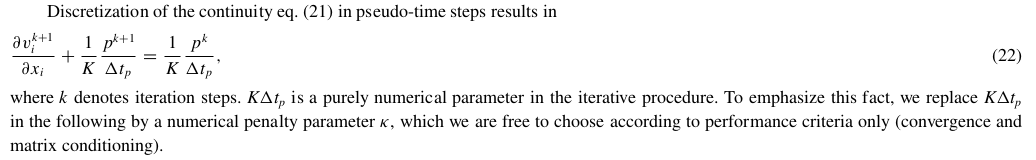
\includegraphics[width=15cm]{images/viscoelasticity/bepo10_ba}}
\[
\vec\nabla\cdot\vec\upnu^{k+1} + \frac{1}{K} \frac{p^{k+1}}{\delta t_p}  = \frac{1}{K} \frac{p^{k}}{\delta t_p}
\Rightarrow
\vec\nabla\cdot\vec\upnu^{k+1} + \frac{1}{\kappa} p^{k+1}  = \frac{1}{\kappa} p^{k}
\]

\fbox{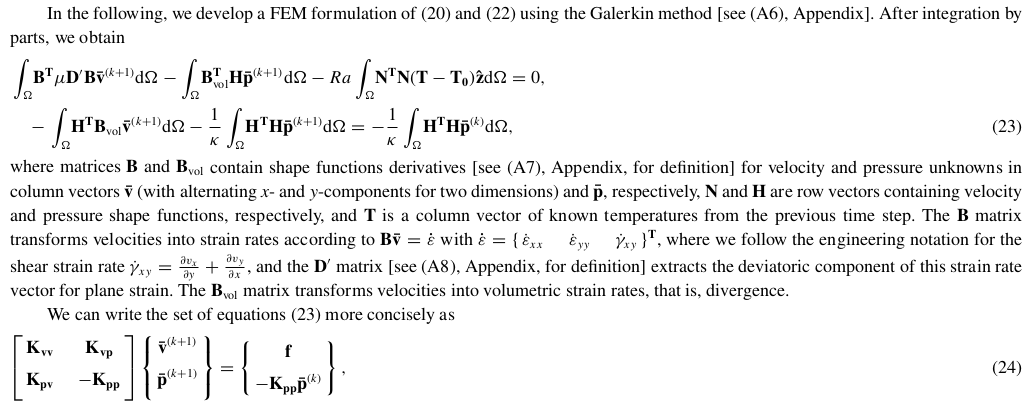
\includegraphics[width=15cm]{images/viscoelasticity/bepo10_bb}}

\fbox{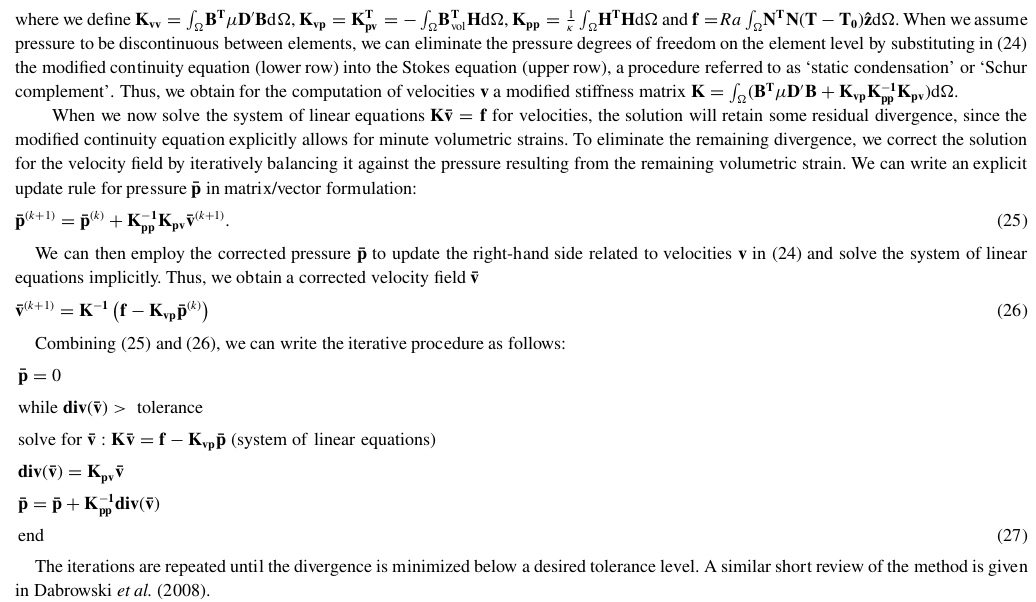
\includegraphics[width=15cm]{images/viscoelasticity/bepo10_c}}

\vspace{.5cm}

``
Use of a viscous rheology might be appropriate for modelling the dynamics of the hot, 
convecting interior of our planet. Yet, when the relatively cold, elastic lithosphere 
is included in the simulation, a viscoelastic rheology is more appropriate. While the 
hot, sublithospheric interior experiences strong deformation on geological timescales 
and thus behaves like a viscous fluid, the lithosphere itself remains relatively
undeformed over long geological times and exhibits the properties of an elastic solid. 
The difference in response of the mantle in the relatively hot sublithospheric interior 
and the relatively cold lithosphere is a consequence of the strong temperature dependence 
of creep activation in mantle rocks (Karato \& Wu 1993). A Maxwell rheology naturally 
combines both viscous and elastic behaviour of mantle rocks, with the transition between 
the two rheological regimes being determined by the temperature-dependent viscosity and 
the timescale considered.
''

\vspace{.5cm}

\fbox{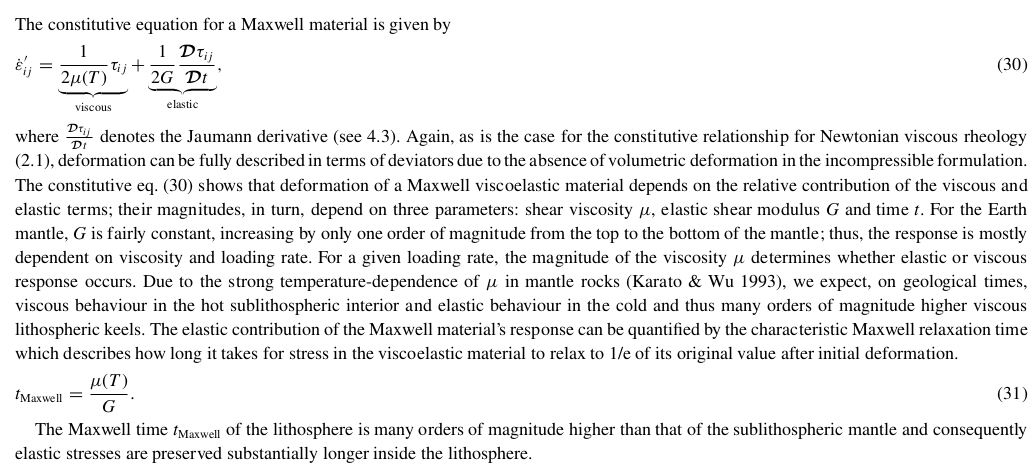
\includegraphics[width=15cm]{images/viscoelasticity/bepo10_d}}



\fbox{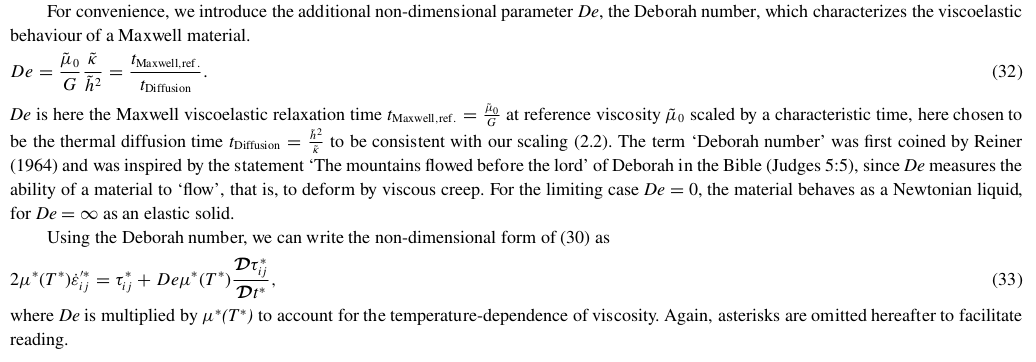
\includegraphics[width=15cm]{images/viscoelasticity/bepo10_e}}

\fbox{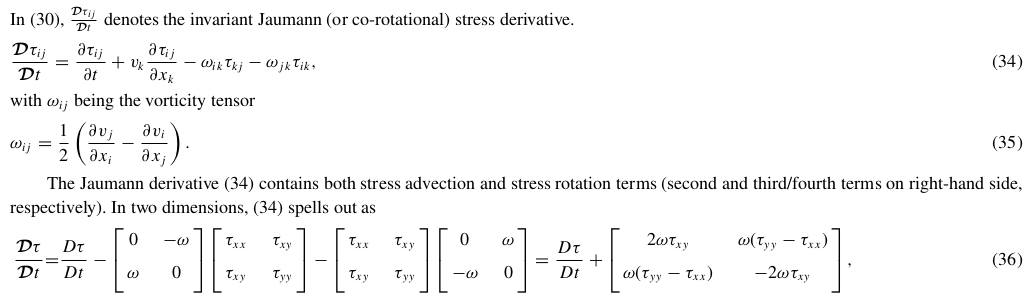
\includegraphics[width=15cm]{images/viscoelasticity/bepo10_f}}

\fbox{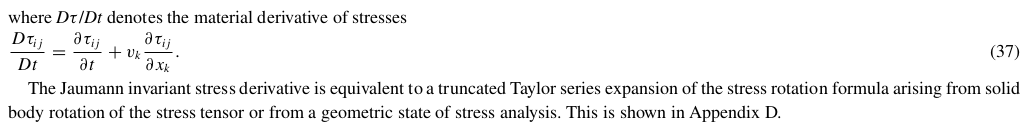
\includegraphics[width=15cm]{images/viscoelasticity/bepo10_g}}


\paragraph{Derivation of Jaumann derivative from stress rotation formula}.

\fbox{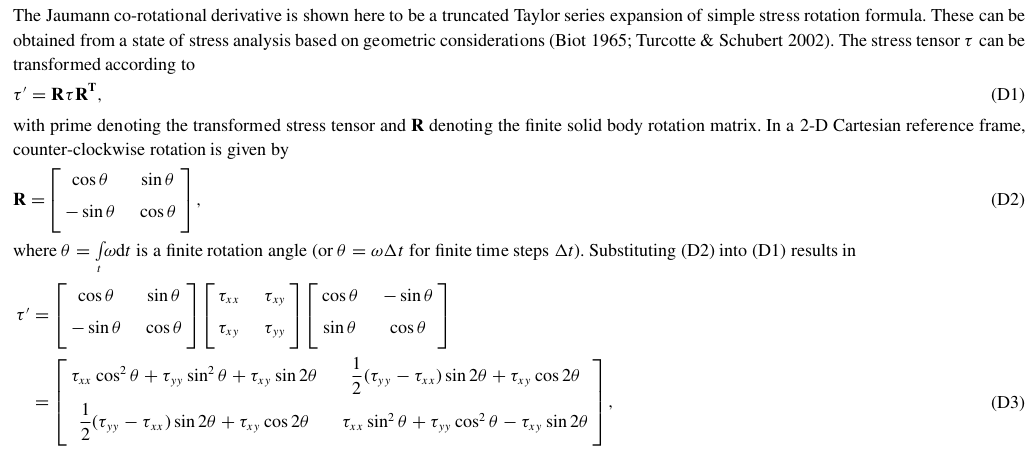
\includegraphics[width=15cm]{images/viscoelasticity/bepo10_h}}\\
\[
{\bm \tau}' = {\bm R} \cdot {\bm \tau} \cdot {\bm R}^T
\]
\[
{\bm R} = 
\left(\begin{array}{cc}
\cos\theta & \sin\theta \\
-\sin\theta  & \cos\theta
\end{array}\right)
\]
\[
\theta = \int_t \omega \; dt \simeq \omega \delta t
\]
\[
{\bm \tau}' = 
\left(\begin{array}{cc}
\cos\theta & \sin\theta \\
-\sin\theta  & \cos\theta
\end{array}\right)
\cdot
\left(\begin{array}{cc}
\tau_{xx} & \tau_{xy} \\
\tau_{xy} & \tau_{yy}
\end{array}\right)
\cdot
\left(\begin{array}{cc}
\cos\theta & -\sin\theta \\
\sin\theta & \cos\theta
\end{array}\right)
\]

\fbox{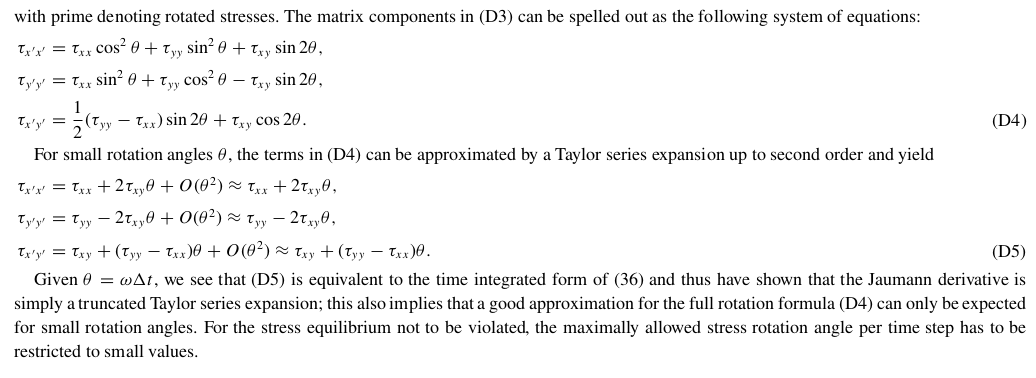
\includegraphics[width=15cm]{images/viscoelasticity/bepo10_i}}

\begin{eqnarray}
\tau_{xx}' &=& \tau_{xx} \cos^2 \theta  + \tau_{yy} \sin^2 \theta  + \tau_{xy} \sin 2 \theta\nn\\
\tau_{yy}' &=& \tau_{xx} \sin^2 \theta  + \tau_{yy} \cos^2 \theta  - \tau_{xy} \sin 2 \theta\nn\\
\tau_{xy}' &=& \frac12 (\tau_{yy}-\tau_{xx}) \sin 2\theta  + \tau_{xy} \cos 2\theta \nn
\end{eqnarray}


\begin{eqnarray}
\tau_{xx}' &=& \tau_{xx}  + 2\tau_{xy} \theta + {\cal O}(\theta^2) \simeq \tau_{xx} + 2\tau_{xy} \theta \nn\\
\tau_{yy}' &=& \tau_{yy}  - 2\tau_{xy} \theta + {\cal O}(\theta^2) \simeq \tau_{yy} - 2\tau_{xy} \theta \nn\\
\tau_{xy}' &=& \tau_{xy} + (\tau_{yy}-\tau_{xx}) \theta  + {\cal O}(\theta^2) \simeq \tau_{xy} + (\tau_{yy}-\tau_{xx}) \theta \nn
\end{eqnarray}

\paragraph{FEM implementation}.

\fbox{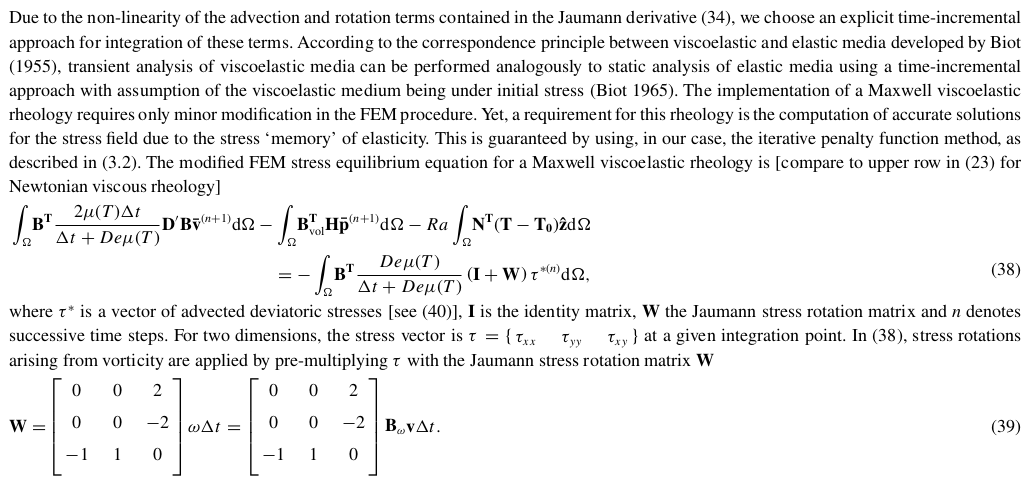
\includegraphics[width=15cm]{images/viscoelasticity/bepo10_j}}

\vspace{4cm}

\fbox{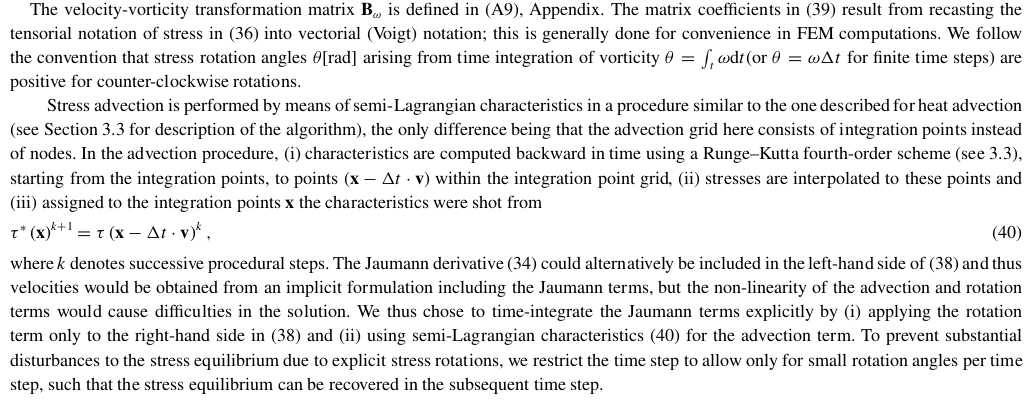
\includegraphics[width=15cm]{images/viscoelasticity/bepo10_k}}




